\documentclass{article}
\usepackage{titlesec}
\usepackage[left=4cm, right=4cm]{geometry}
\usepackage{palatino}%Font
\usepackage{graphicx}
\usepackage{wrapfig}
\usepackage{float}
\usepackage{subcaption}
\usepackage{enumerate}
\usepackage{parskip}
\usepackage{multirow}
\usepackage{multicol}
\setlength{\columnsep}{-50pt}
\usepackage{listings}
\lstset{basicstyle=\ttfamily,
	breaklines=true}
\usepackage{fancyvrb}
\usepackage{booktabs}
\usepackage{amsthm}
\usepackage{amssymb}
\usepackage{amsmath}
\usepackage[htt]{hyphenat}
\usepackage{cancel}
\usepackage{tikz}
\usepackage{tikz-cd}
\usepackage{tikz-3dplot}
\usepackage{xcolor}
\usepackage[bookmarks,bookmarksopen,bookmarksdepth=3]{hyperref}
\hypersetup{
	colorlinks=true,
	urlcolor=blue,
	linkcolor=magenta,
	citecolor=blue,
	filecolor=blue,
	urlbordercolor=white,
	linkbordercolor=white,
	citebordercolor=white,
	filebordercolor=white
}

\usepackage{etoolbox}
\usepackage{cleveref}
\crefname{figure}{fig.}{figs.}
\Crefname{figure}{Fig.}{Figs.}
\renewcommand{\figurename}{Fig.}
\usepackage[title,titletoc]{appendix}

%Bold references
%\usepackage{xpatch}
%\makeatletter
%\xpatchcmd{\@cref}{\begingroup}{\begingroup\bfseries}{}{}
%\makeatother
%\captionsetup[figure]{labelfont=bf}

\theoremstyle{definition}

\newtheorem*{defn}{Definition}
\newtheorem*{lem}{Lemma}
\newtheorem*{rem}{Remark}
\newtheorem*{thm}{Theorem}
\newtheorem*{prop}{Proposition}
\newtheorem*{claim}{Claim}

\newcommand{\E}{\mathbb{E}}
\newcommand{\R}{\mathbb{R}}
\newcommand{\Z}{\mathbb{Z}}
\newcommand{\N}{\mathbb{N}}
\newcommand{\C}{\mathbb{C}}
\newcommand{\Q}{\mathbb{Q}}
\newcommand{\s}{\mathbb{S}}
\newcommand{\PP}{\mathbb{P}}
\newcommand{\p}{\mathcal{P}}
\newcommand{\T}{\mathcal{T}}
\DeclareMathOperator{\Id}{Id}
\DeclareMathOperator{\img}{img}
\DeclareMathOperator{\Fix}{Fix}
\DeclareMathOperator{\Stab}{Stab}

%Referencias
\usepackage[style=numeric-comp, backend=bibtex, doi=false, isbn=false, natbib=true]{biblatex}
\addbibresource{bib.bib}


\title{A new chiral 4-polytope}
\author{\\Daniel González Casanova Azuela}
\date{}

\def\changemargin#1#2{\list{}{\rightmargin#2\leftmargin#1}\item[]}
\let\endchangemargin=\endlist

\begin{document}
\thispagestyle{empty}
\begin{figure}[H]
	\centering
	
\includegraphics[width=0.3\linewidth]{fig0}
\end{figure}

\begin{center}
	\textbf{UNIVERSIDAD NACIONAL AUTÓNOMA DE MÉXICO}
	
	PROGRAMA DE MAESTRÍA Y DOCTORADO EN CIENCIAS MATEMÁTICAS Y DE LA ESPECIALIZACIÓN EN ESTADÍSTICA APLICADA
	
	\vspace{2cm}
	{\Large Two new chiral 4-polytopes in $\E^4$}
	\vspace{1.2cm}
	
	TESINA
	
	QUE PARA OPTAR POR EL GRADO DE:
	
	MAESTRO EN CIENCIAS
	\vspace{1.2cm}
	
	PRESENTA:
	
	DANIEL GONZÁLEZ CASANOVA AZUELA
	\vspace{1.2cm}
	
	DIRECTOR:
	
	JAVIER BRACHO CARPIZO
	
	INSTITUTO DE MATEMÁTICAS, UNAM
	\vspace{1.2cm}
	
	CIUDAD DE MÉXICO, OCTUBRE DE 2023
\end{center}

\clearpage

\begin{changemargin}{3.3cm}{0cm} 
%\section*{Agradecimientos}

\vspace*{4cm}

{\Large\textbf{Agradecimientos}}
\vspace{1cm}

A mis queridos tutores Roli e Isabel por transmitirme tanta emoción. A Bris por ser un modelo a seguir. Al equipo de politoperes por todo su cariño. A Vinicio Gómez por estar siempre. A mi familia.
\end{changemargin}
\clearpage
	
	
	\section*{Summary}
	In the context of skeletal geometric complexes, chiral polytopes are those with maximal rotational symmetry but no reflection symmetry. We show that the natural rotation about the base edge in two of the chiral polyhedra from \cite{petcox} yields, in each case, a chiral 4-polytope in $\E^4$. Both polytopes are shown to be combinatorially chiral.
	
	\vspace{1cm}
	%	\phantomsection
		\tableofcontents
		\clearpage
	\section{Introduction}
	Despite polygons and polyhedra being basic concepts in mathematics,
	% studied since antiquity,
	 it is not at all obvious what these words exactly mean. Chiral polytopes arise from the so-called skeletal approach, where polygons and their higher-dimensional analogues are introduced as 1-dimensional complexes, with no need of an enclosed surface or solid.
	
	Such definition allows for symmetric structures otherwise unseen, an example of which are chiral polytopes. While the symmetry group of a regular polyhedron acts transitively on the set of flags, a polyhedron is geometrically chiral when its symmetry group has two orbits on the flags and adjacent flags are in distinct orbits. This captures the idea of maximal rotational symmetry but no reflection symmetry.
	
	Chiral polyhedra first appeared in 2005, when Schulte classified those realisable in $\E^3$, non of which is finite nor its faces are contained in planes (see \cite{chiral-polyhedra-i,chiral-polyhedra-ii}). The first example of a chiral 4-polytope in $\E^4$, so-called Roli's cube, was constructed in 2014 by Bracho, Hubard and Pellicer \cite{rolis-cube}. It was later shown that the facets of this polytope belong to a broader family of chiral polyehdra with helical faces in $\mathbb{S}^3$ \cite{petcox}.
	
	In this thesis we show that the natural rotation about the base edge in two such spherical polyhedra successfully yields, in each case, a chiral 4-polytope. Their combinatorial structures are then shown to be chiral as well---something that does not occur for their facets, which are combinatorially regular.
	
	Proofs are given by GAP programs in which the abstract and geometric structures are compared. Geometric realizations are based on the reflection matrices used in \cite{petcox}. All programs used are available online (see \Cref{app:A}).
	
	\section{Historical background}
	We begin with a brief historical discussion on the concept of polytope.
	
	We cannot find a moment in history when triangles and squares came to attract the attention of humans. Later, when mathematics became an established discipline, simple polygons and polyhedra were thoroughly studied: the first proposition in Euclid's elements is the construction of a regular triangle, and the last book is devoted to the study of Platonic Solids \cite{euclid}.
	
	After the greeks, the definition of polygon remained essentialy unchanged for many centuries. The first account of an important difference dates to the XIV century, when an Archbishop of Canterbury investigated star polygons \cite{abstract-polytopes}.
	These are essentially different by being non-convex: their edges intersect in points that are not vertices of the polygon. They may be, however, studied by their symmetry properties just like regular convex polygons.
	
	Regular star polyhedra are the natural generlization of regular star polygons to euclidean 3-space. They take us to the XVII century with Johannes Kepler, who studied the two whose faces are star polygons (pentagrams). Their duals, whose faces are convex but their vertex-figures are not, where studied in 1809 by Louis Poinsot \cite{abstract-polytopes}.
	
	Higher-dimensional polytopes were first studied in the XIX century, when Ludwig Schläfli found all the regular polytopes whose symmetry groups are generated by reflections in hyperplanes in euclidean spaces \cite{abstract-polytopes}.
	
	Next in history is Coxeter, who, among many other results, classiffied all discrete euclidean reflection groups. In the 1930's him and Petrie redefined the concept of polytope by letting them have infinite faces, thus finding three more regular polyhedra in $\E^3$ \cite{regular-skew}. These have non-planar vertex-figures.
	
	Fourty years later, in 1977, Grünbaum once again reintroduced polytopes, this time permitting the faces to be non-planar \cite{grunbaum}. The list of regular polyhedra in $\E^3$ was extended to 18 in the finite case and 48 in total \cite{regular-ordinary}. All but one were classified by Grünbaum, the remaining one and the completeness of the list are due to Dress \cite{Dress1981,Dress1985}.
	
	The study of the underlying combinatorial structure of polytopes led to the concept of abstract polytope. In 1967 McMullen studied the lattice of faces of a polytope and compared its automorphisms with geometric symmetries \cite{mcmullen-combinatorially}. In Grümbaum's \cite{grunbaum-regularity}, the term \textit{polystroma} (stroma=stratum, layer) is defined to mean an abstract partially order structure resembling the face lattice of a polytope.
	
	Chiral polytopes were first studied in this abstract sense, a general theory first given in 1991 by Schulte and Weiss \cite{schulte-chiral}. Back to geometry, skeletal chiral polyhedra in $\E^3$ were studied in \cite{chiral-polyhedra-i,chiral-polyhedra-ii}, and the first example of a skeletal chiral 4-polytope in $\E^4$ is Roli's cube from \cite{rolis-cube}.
	
	\section{Skeletal polyhedra and 4-polytopes in $\E^4$}\label{sec:skeletal}
	Now we give formal definitions and basic results.
	
	A \textit{skeletal polyhedron} in $\E^4$ consists of \textit{vertices} (points in $\E^4$), \textit{edges} (segments between vertices) and \textit{faces} (cycles on the graph determined by the vertices and edges) such that:
	\begin{enumerate}[\itshape(i)]
		\item every edge belongs to two faces,
		\item the graph determined by the vertices and edges is connected,
		\item every compact subset of $\E^4$ meets finitely many edges, and
		\item the \textit{vertex-figure}, defined as follows, is a connected graph. For any vertex $v$, the vertices of the vertex-figure are the neighbours of $v$ and the edges are segments joining any two neighbours that are both in some face.
	\end{enumerate}
	A \textit{skeletal 4-polytope} in $\E^4$ consits of vertices, edges, faces and \textit{cells} (skeletal polyhedra), such that
	\begin{enumerate}[\itshape(i)]
		\item every face belongs to two cells,
		\item the graph determined by the vertices and the edges is connected,
		\item every compact subset of $\E^4$ meets finitely many edges, and
		\item the vertex-figure at every vertex is a skeletal polyhedron.
		\end{enumerate}
	
	Hereafter we omit the term "skeletal" when the context permits it. If $\p$ is a 4-polytope, the set of vertices, edges, faces and cells is a partial order with respect to inclusion. We say two such elements are \textit{incident} if they are comparable. This poset is called the \textit{abstract polytope associated to $\p$}. As we shall see, 4-polytopes defined as above are realizations of abstract polytopes in the sense of \cite{abstract-polytopes} and \Cref{sec:abstract-defs}.
	
	A \textit{flag} is a 4-tuple of incident vertex, edge, face and cell. Two flags are \textit{adjacent} when they differ by only one element. We call two flags \textit{0-adjacent} if they differ by a vertex, \textit{1-adjacent} if they differ by an edge, \textit{2-adjacent} if they differ by a face and \textit{3-adjacent} if they differ by a cell.
	
	A \textit{symmetry} of $\p$ is an isometry of $\E^4$ that preserves it set-wise. The group of symmetries of $\p$ will be denoted by $G(\p)$. We call $\p$ \textit{regular} if $G(\p)$ acts transitively on the set of flags, and \textit{chiral} if $G(\p)$ induces two orbits on flags so that adjacent flags are on different orbits. In fact, whether $\p$ is regular or chiral, its symmetry group acts transitively on the sets of vertices, edges, faces and cells.
	

	
\section{Abstract 4-polytopes}\label{sec:abstract-defs}
	The theory of abstract polytopes is an essential tool for our work. In this section we state basic results and constructions upon which our proofs are based. To avoid using the word 'abstract' in every definition, we use the same words as in the previous section to mean different objects. All polytopes are abstract up to \Cref{subsec:realizations}, where they are precisely distinguished.
	
	An \textit{abstract $4$-polytope} is a partial order $\p$ that satisfies the following properties (P1) to (P4). The elements of $\p$ are called \textit{faces} and the maximally ordered subsets (chains) are called \textit{flags}.
	\begin{enumerate}
		\item[(P1)]\label{P1} $\p$ contains a minimal face and a greatest face, denoted respectively by $F_{-1}$ and $F_4$.
		\item[(P2)]\label{P2} Flags contain $6$ elements, including $F_{-1}$ and $F_4$.
	\end{enumerate}
	Since every element in a poset is in some chain, we may assign to every face a number from $-1$ to $4$. Such is the \textit{rank function} of $\p$. We say that two flags are \textit{$i$-adjacent} if they differ only by a face of rank $i$.
	\begin{enumerate}
		\item[(P3)]\label{P3} $\p$ is \textit{strongly flag connected} in the following sense. For any two distinct flags $\Phi$ and $\Psi$ there is a sequence
		\[\Phi=\Phi_0,\Phi_1,\ldots,\Phi_k=\Psi\]
		so that $\Phi_{i-1}$ and $\Phi_i$ are adjacent and $\Phi\cap\Psi\subset\Phi_i$ for all $i$.
		\item[(P4)]\label{P4} If $F$ and $G$ are a $(i-1)$-face and a $(i+1)$-face with $F<G$ and $0\leq j\leq2$, then there are exactly two $i$-faces $H$ such that $F<H<G$.
	\end{enumerate}
	
		\subsection{Regular and chiral abstract 4-polytopes}
	Now we study regular 4-polytopes and their automorphism groups. An \textit{automorphism} of $\p$ is a bijection of the polytope that preserves incidence, and we denote the automorphism group by $\Gamma(\p)$. $\p$ is called \textit{regular} if $\Gamma(\p)$ is transitive on flags.
	
	For a regular polytope $\p$ and some distinguised flag $\Phi$, there exists a unique involutory automorphism $\rho_j$ of $\p$ such that $\Phi\rho_i=\Phi^i$ for $i=0,1,2,3$ (Prop. 2B4, \cite{abstract-polytopes}). These are called the \textit{distinguished generators} of $\Gamma(\p)$ and satisfy that 
	\begin{equation}\label{eq:string-reg}
			(\rho_i\rho_j)^{p_{ij}}=\Id\text{ when } |i-j|\geq2\
	\end{equation}
	for $i,j=0,1,2,3$ (prop. 2B11 \cite{abstract-polytopes}). The numbers $p_i:=p_{i-1}p_i$ form the \textit{Schläfli type} $\{p_1,p_2,p_3\}$ of $\p$. The distinguished generators also satisfy 
	\begin{equation}\label{eq:int-reg}
		\langle \rho_i|i\in I\rangle\cap\langle\rho_j|j\in J\rangle=\langle\rho_i\in I\cap J\rangle\qquad\text{for }I,J\subseteq\{0,1,2,3\}
	\end{equation}
	which we call the \textit{intersection property} (prop. 2B10 \cite{abstract-polytopes}). Any group $\Gamma$ generated by the involutions $\rho_0$ to $\rho_3$ satisfying \cref{eq:string-reg,eq:int-reg} is called a \textit{C-string group}. We have established that $\Gamma(\p)$ is one such group.
	
	Conversely, we may construct a regular abstract $4$-polytope from a C-string group $\Gamma$. Define $\Gamma_j:=\langle\rho_j|i\neq j\rangle$ and $\Gamma_{-1}=\Gamma_4=\Gamma$, and take the set of $i$-faces to be the set of right cosets $\Gamma_i\varphi$ for $\varphi\in\Gamma$. Then there is an order relation with respect to which the set of all faces is a regular $4$-polytope whose automorphism group is $\Gamma$ (thm. 2E11, \cite{abstract-polytopes}).
	
	\vspace{.5cm}
	
	Now we revise the analogue construction for chiral polytopes. An abstract 4-polytope $\p$ is called \textit{chiral} if $\Gamma(\p)$ induces two orbits on flags and two adjacent flags are in different orbits.
	
	First observe that by defining $\sigma_i:=\rho_{i-1}\rho_i$ for the distinguished generators of a regular polytope with bipartite flags, it holds that
	\begin{equation}\label{eq:chiral-rels}
		\begin{aligned}
			\sigma_1^{p_1}=\sigma_2^{p_2}&=\sigma_3^{p_3}=\Id\\
			(\sigma_1\sigma_2)^2=(\sigma_1\sigma_2&\sigma_3)^2=(\sigma_2\sigma_3)^2=\Id
		\end{aligned}
	\end{equation}
	for some positive integers $p_1$, $p_2$ and $p_3$ (see \cite{schulte-chiral}).
	
	The group generated by these elements is called the \textit{rotation subgroup} of $\p$, denoted by $\Gamma^+(\p)$. For chiral polytopes this will be the whole group: if $\p$ is chiral, $\Gamma(\p)$ is generated by three automorphisms $\sigma_1,\sigma_2$ and $\sigma_3$ that satisfy \cref{eq:chiral-rels} (prop. 3, \cite{schulte-chiral}).
	
	To construct a chiral or regular abstract polytope from a group we must also require some sort of intersection property. It will suffice that
	\begin{equation}\label{eq:chiral-int}
		\begin{aligned}
			\langle\sigma_1\rangle\cap\langle\sigma_2\rangle=\{\Id\}&=\langle\sigma_2\rangle\cap\langle\sigma_3\rangle\\
			\langle\sigma_1,\sigma_2\rangle\cap\langle\sigma_2,&\sigma_3\rangle=\langle\sigma_2\rangle.
		\end{aligned}
	\end{equation}
	Let $\Gamma=\langle \sigma_1,\sigma_2,\sigma_3\rangle$ be a group satisfying both \cref{eq:chiral-rels,eq:chiral-int}. Define
	\begin{align*}
		\Gamma^0=\langle\sigma_2,\sigma_3\rangle,\quad
		\Gamma^1=\langle \sigma_3,\sigma_1\sigma_2\rangle,\quad
		\Gamma^2=\langle &\sigma_1,\sigma_2\sigma_3\rangle,\quad
		\Gamma^3=\langle \sigma_1,\sigma_2\rangle,\\
		\text{and}\quad\Gamma_{-1}=\Gamma^4=\Gamma,
	\end{align*}
	and take the $i$-faces to be the right cosets $\Gamma_i\varphi$ for $\varphi\in\Gamma$. Again, the set of all faces admits a partial order with respect to which it is a chiral or a regular abstract 4-polytope $\p$ such that $\Gamma^+(\p)=\Gamma$ (thm. 1 and lem. 11, \cite{schulte-chiral}).
	
	In this construction we may distinguish chiral from regular abstract 4-polytopes as follows. $\Gamma^+(\p)$ is of index 2 in $\Gamma(\p)$ if and only if there exists an involutory automorphism $\rho:\Gamma\to \Gamma$ such that
	\begin{equation}\label{eq:combinatorially-chiral}
		\rho(\sigma_1)=\sigma_1^{-1},\quad \rho(\sigma_2)=\sigma_1^2\sigma_2\quad\text{and}\quad \rho(\sigma_3)=\sigma_3,
\end{equation}
	in which case $\p$ cannot be chiral (thm. 1, \cite{schulte-chiral}).

\vspace{10pt}

	\subsection{Realizations}\label{subsec:realizations}
	Now we review the relationship between abstract and skeletal polytopes as defined in \Cref{sec:skeletal}.
	
	A \textit{realization} of an abstract polytope $\p$ is a map $\beta$ from the set of abstract 0-faces $\p_0$ into $\E^4$, so that the set $V_0:=\p_0\beta$ is the set of geometric vertices. All other geometric faces are defined by functions from the set of abstract $i$-faces $\p_i$ to some nested power set of the geometric vertex set: edges are sets of vertices, faces are sets of edges and so on.
	
	Formally, for $i=1,2,3$, $\beta$ induces a surjection $\beta_i:\p_i\to V_i$, where $V_i$ is thought as the set of geometric $i$-faces, consisting of the elements ${F\beta_i:=\{G\beta_{i-1}|G\in\p_{i-1}\text{ and }G\leq F\}}$ for $F\in\p_i$ (thm. 5A1, \cite{abstract-polytopes}). For example, an abstract edge $E\in\p_1$ is mapped to a set consisting of the two points (there's only two by (P4)) in $\E^4$ whose preimages are abstract vertices smaller than $E$ in $\p$.

	
%	Let the set of $i$-faces of an abstract polytope $\p$ be denoted by $\p_i$. Define $V_0:=\p_0\beta$ and $V_j$ to be the set consisting of elements of the form $F\beta_j:=\{G\beta_{j-1}|G\in\p_{j-1}\text{ and }G\leq F\}$ for $F\in\p_j$ and any $j$. Then $\beta$ induces surjections $\beta_j:\p_j\to V_j$. A realization is \textit{faithful} when each $\beta_j$ is a bijection.

	Of course, we expect the number of $i$-faces of the abstract and geometric structures to be the same. A realization is \textit{faithful} if every $\beta_i$ is a bijection.
	
	We also expect automorphisms to correspond with isometries of $\E^4$. A realization is \textit{symmetric} when every automorphism of $\p$ induces a permutation of $V_0$, which in turn determines a unique isometry of $\E^4$ (if the vertex set affinely spans $\E^4$). Then these isometries are an euclidean representation of $\Gamma(\p)$.
	
	Conversely, given an euclidean representation of the automorphism group $\Gamma(\p)$ of an abstract 4-polytope, we obtain a realization by \textit{Wythoff's construction} as follows.
	
	For the regular case, let $\langle R_0, R_1,R_2,R_3\rangle$ be an euclidean representation of the automorphism group of a regular abstract 4-polytope $\p$. Should there be any, define a point $v\in\E^4$ that is fixed by $R_1$, $R_2$ and $R_3$ but not by $R_0$ as the base vertex and take the orbit of $v$ for the geometric vertex-set of a realization. Further, define the base edge $e=v\langle R_0\rangle$, the base face $f=e\langle R_0,R_1\rangle$ and the base cell $c=f\langle R_0,R_1,R_2\rangle$ for a geometric base flag.
	
	Now let $\langle S_1,S_2,S_3\rangle$ be a representation of the automorphism group, or rotation subgroup, of a chiral or regular abstract 4-polytope, respectively. For a geometric base vertex choose any point that is fixed by $S_2$ and $S_3$ but not by $S_1$. The orbit of this point is the geometric vertex-set of a realization. For a geometric flag we define the base edge as $e=v\langle S_1S_2\rangle$, or equivalently, as $e=\{v,vS_1^{-1}\}$ since $S_1^{-1}=R_1R_0$ when $\p$ is regular. Define the base face as $f=e\langle S_1\rangle$ and the base cell as $c=f\langle S_1,S_2\rangle$.
	
	While it is true that realizations of 4-polytopes are mere clouds of points, they are no generalization of skeletal polytopes---the segment between vertices is still taken to be flat. Save this technical difference, it is straightforward to check that a regular or chiral skeletal 4-polytope as defined in \Cref{sec:skeletal} is a faithful and symmetric realization of the abstract 4-polytope related to it.
	
	\vspace{.5cm}
	
	It remains only to formally define star polytopes. Following Section 7D from \cite{abstract-polytopes}, we say a faithfully realized abstract 4-polytope is \textit{classical} if every geometric $i$-face has dimension $i$ (its affine hull is $i$-dimensional). For any such geometric regular polytope, we may write its generating hyperplane reflections as
	\[R_i=\{x\in\E^4|\langle x,u_i\rangle=0\}\]
	for some unit vectors $u_i$. Then $\langle u_i,u_j\rangle=0$ for $|i-j|\geq2$, and, since $\langle R_i,R_j\rangle$ is a finite group, there is a rational number $p_i$ such that $\langle u_{i-1},u_i\rangle=\cos(\pi/p_i)$. We define the \textit{Shläfli type} of this polytope as $\{p_1,p_2,p_3\}$ and call it a \textit{star 4-polytope} if any of the $p_i$ is not an integer. Of course, the definition for polyhedra is analogous.

	\section{A realization of $\left\{\frac{5}{2},3,5\right\}$}
	Out first chiral polytope will have the same vertices and edges as the star 4-polytope $\left\{\frac{5}{2},3,5\right\}$. We shall start by constructing $\left\{\frac{5}{2},3,5\right\}$ from a given realization of $\{3,3,5\}$. To this end we first express the generating reflections of $\left\{\frac{5}{2},3,5\right\}$ in terms of those of $\{3,3,5\}$. Then we prove they generate a C-string group, which in turn yields an abstract polytope. Finally we show it is realized as $\left\{\frac{5}{2},3,5\right\}$.
	
	Our construction is based in the following observations. In the regular star polyhedron $\left\{\frac{5}{2},3\right\}$ the edges intersect at points that are not vertices, and the convex hull of these intersections is a regular icosahedron. The vertex-figure of $\{3,3,5\}$ is also a regular icosahedron. Further, the vertices of $\left\{\frac{5}{2},3,5\right\}$ must be the same as those of $\{3,3,5\}$ (\cite{abstract-polytopes}, p. 212).
	
	We are thus inclined to look for a copy of $\left\{\frac{5}{2},3\right\}$ within $\{3,3,5\}$ by taking the vertex-figure icosahedron of some vertex and at each of its faces consider the ajacent tetrahedron that is not contained in the interior of the icosahedron. We may visualize this by stereographically projecting the vertices and taking the convex hull of each tetrahedron as in \cref{fig:fig1}.
	
	\begin{figure}[h]
	\centering
	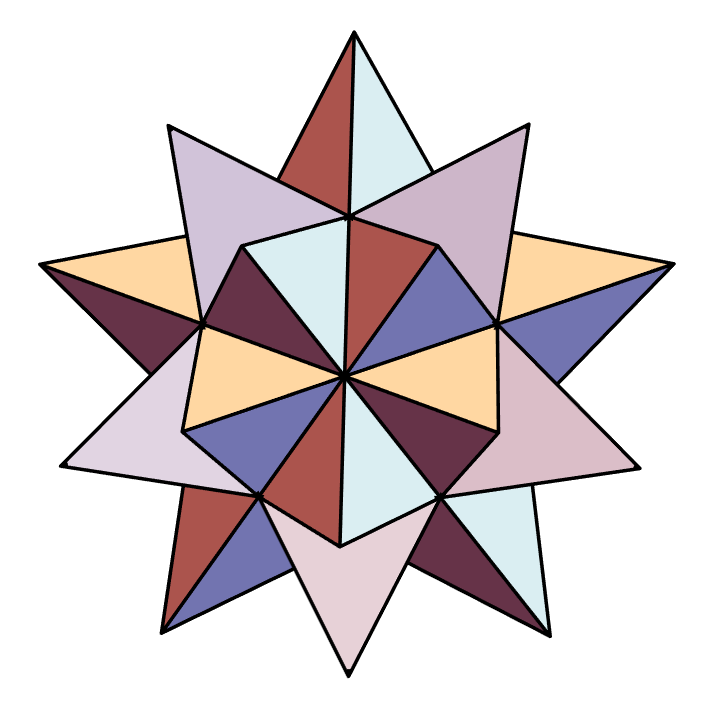
\includegraphics[width=0.7\linewidth]{fig1}
	\caption{The base cell of $\left\{\frac{5}{2},3,5\right\}$.}
	\label{fig:fig1}
	\end{figure}
	
	Notice that an edge of $\left\{\frac{5}{2},3\right\}$ is composed of three edges of $\{3,3,5\}$. Choosing a geometric flag for $\left\{\frac{5}{2},3,5\right\}$ ammounts to selecting an incident vertex, edge and face within this figure, which is the base cell.  We define the generating reflections of the symmetry group of $\left\{\frac{5}{2},3,5\right\}$ with respect to the base flag as follows. Call the base vertex $w_0$, the centroid of the base edge  $w_1$, the centroid of the base face  $w_2$ and the centroid of the base cell  $w_3$. The mirror of the reflection $P_i$ is the hyperplane through the origin and the $w_j$ such that $j\neq i$.
	
	There is a choice of base flag for $\{3,3,5\}$ for which the generating reflections $R_0$ to $R_3$ result the following relations, that we shall use as definitions:
	\begin{gather*}
		P_0=R_0,\qquad P_2=R_3,\qquad P_3=R_2\\
		P_1=R_1R_2R_3R_2R_1R_0R_1R_2R_3R_2R_1
	\end{gather*}
	To construct a realization of $\left\{\frac{5}{2},3,5\right\}$ we first suppose that $R_0$ to $R_3$ are the distinguished generators of the abstract polytope $\{3,3,5\}$. That is, they satisfy the relations
	\[R_i^2=(R_0R_1)^3=(R_1R_2)^3=(R_2R_3)^5=(R_0R_2)^2=(R_0R_3)^2=(R_1R_3)^2=\Id\]
	for all $i$ and the intersection property. It has been confirmed that
		\[P_i^2=(P_0P_1)^5=(P_1P_2)^3=(P_2P_3)^5=(P_0P_2)^2=(P_0P_3)^2=(P_1P_3)^2=\Id\]
	for all $i$, and that the intersection property holds (see \Cref{app:1}). Then the abstract polytope generated by $P_0$ to $P_3$ is $\{5,3,5\}$.
	
	Using a particular realization of $\{3,3,5\}$, we may explicitly find the base vertex for $\left\{\frac{5}{2},3,5\right\}$ (see \Cref{app:coords}). Then Wythoff's construction yields a realization that we expect to be faithful and symmetric. Faithfullness follows by comparing the number of $i$-faces of the abstract polytope and the realization (see \Cref{app:1,app:2}). Symmetry follows from the fact the vertex-set of both $\{3,3,5\}$ and $\left\{\frac{5}{2},3,5\right\}$ is the same.
	
	Since the $R_i$ are hyperplane reflections, we have a classical polytope as defined in \Cref{subsec:realizations} (see \cite{mcmullen-4dimensional}). The only such polytopes in $\mathbb{E}^4$ arising from the abstract regular polytope $\{5,3,5\}$ are the star 4-polytopes $\left\{\frac{5}{2},3,5\right\}$ and $\left\{5,3,\frac{5}{2}\right\}$ (thm. 7D13 \cite{abstract-polytopes}). However, the rotation about the edge in this polytope is the reverse of that of $\{3,3,5\}$, so that it cannot be of type $\frac{5}{2}$. This completes the proof that we have constructed $\left\{\frac{5}{2},3,5\right\}$.
	
	\section{A chiral 4-polytope from $\left\{\frac{5}{2},3,5\right\}$}
	To construct a chiral 4-polytope within $\left\{\frac{5}{2},3,5\right\}$, let
		\[S_1=P_0P_1P_3P_2,\qquad S_2=P_2P_1,\quad\text{and}\quad S_3=P_3P_2.\]
	Then
	\begin{equation}\label{eq:string-chiral}
		S_1^{12}=S_2^3=S_3^5=(S_1S_2)^2=(S_1S_2S_3)^2=(S_2S_3)^2=\Id
	\end{equation}
	and \cref{eq:chiral-int} holds (see \Cref{app:1}). It follows that the group generated by $S_1$ to $S_3$ yields either a regular or a chiral abstract polytope.
	
	For a realization by Wythoff's construction define the base vertex to be the same as the one that was used for $\left\{\frac{5}{2},3,5\right\}$. Such a choice and the fact that the group $\langle S_1,S_2,S_3\rangle$ a subgroup of $\langle P_0,P_1,P_2,P_3\rangle$ make the realization symmetric. Again, by comparing the number of $i$-faces in the abstract and geometric polytopes, our realization is seen to be faithful.
	
	The definitions of $S_1$ and $S_2$ are as in  \cite{petcox}, so that the cells are copies of the chiral polyhedron denoted as $H_1(\left\{5,3,\frac{5}{2}\right\})$. In fact, chirality in our 4-polytope follows from the chirality of the cells, since any symmetry sending a flag to its $i$-th adjacent is also a symmetry of the cell.
	
	We have shown this structure to have 120 vertices, 720 edges, 300 faces and 50 cells. Every face has 12 vertices and edges arranged in helical fashion as shown in \cite{petcox} (see \cref{fig:12}). In virtue of such arrangement we denote this polytope by $\left\{\frac{12}{1,5},3,5\right\}$.
	
	
	We now show this structure satisfies \textit{(i)-(iv)} in our definition of skeletal 4-polytope. By the realization being faithful and symmetric, conditions \textit{(i)} and \textit{(ii)} follow from (P4) and (P3), respectively. For \textit{(iii)} notice the vertex figures are icosahedra, which follows from Wythoff's construction on any vertex adjacent to the base vertex by the group $\langle S_2,S_3\rangle$. Finally, \textit{(iv)} is immediate from the finiteness of the group. This concludes the proof that we have constructed a chiral 4-polytope.
	
%	We may also show \textit{(i)} in a slightly more geometric way. It has been shown in  \texttt{geometric.txt} that for the base face $f$,
%	\begin{equation*}\label{ec:stab-face}
%		\Stab_{\langle S_1,S_2,S_3\rangle}(f)=\langle S_1,S_2S_3\rangle,
%	\end{equation*}
%	which implies that every face belongs to exactly two cells. In fact, since $S_1$ fixes the base cell and $S_2S_3$ an involution, if any cell has $f$ as a face, we may map it to the base cell by a transformation fixing $f$.
	
	Further, it was found that there exists no automorphism $\rho$ of the group generated by the $S_i$ that satisfies \cref{eq:combinatorially-chiral}, so that the abstract polytope associated to $\left\{\frac{12}{1,5},3,5\right\}$ is combinatorially chiral (see \Cref{app:1}).
	
	

\begin{figure}[H]
	\begin{center}
			\centering
			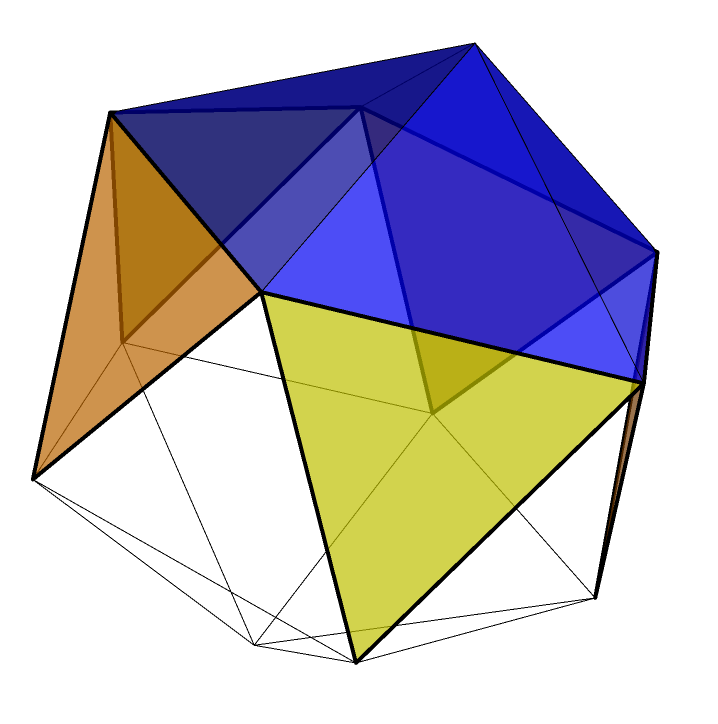
\includegraphics[width=1\linewidth]{fig2}
			\caption{Stereographic projection of the base face of  $\left\{\frac{12}{1,5},3,5\right\}$. We also show the base face of $\left\{\frac{5}{2},3,5\right\}$}\label{fig:12}
	\end{center}
\end{figure}

	
	\section{A chiral 4-polytope from $\left\{5,3,\frac{5}{2}\right\}$}
	For the dual star polytope $\left\{5,3,\frac{5}{2}\right\}$ we simply define
	\[Q_0=P_3,\qquad Q_1=P_2\qquad Q_2=P_3,\quad\text{and}\quad Q_3=P_0\]
	and apply Wythoff's construction on the centroid of the base cell of $\left\{\frac{5}{2},3,5\right\}$. This yields a realization of $\left\{5,3,\frac{5}{2}\right\}$.
	
	Analogue definitions for the $S_i$ as in the last section also satisfy \cref{eq:string-chiral} and \cref{eq:chiral-int}, so that we have another abstract 4-polytope that is, in fact, the same as the (abstract) one constructed before.
	
	Wythoff's construction on the base vertex then yields a symmetric and faithful realization of a chiral 4-polytope whose cells are copies of $H_0(\left\{5,3,\frac{5}{2}\right\})$ from \cite{petcox}. We call it $\left\{\frac{12}{1,5},3,\frac{5}{2}\right\}$.
	
\begin{figure}[H]
	\begin{center}
		\begin{subfigure}{\linewidth}
			\centering
			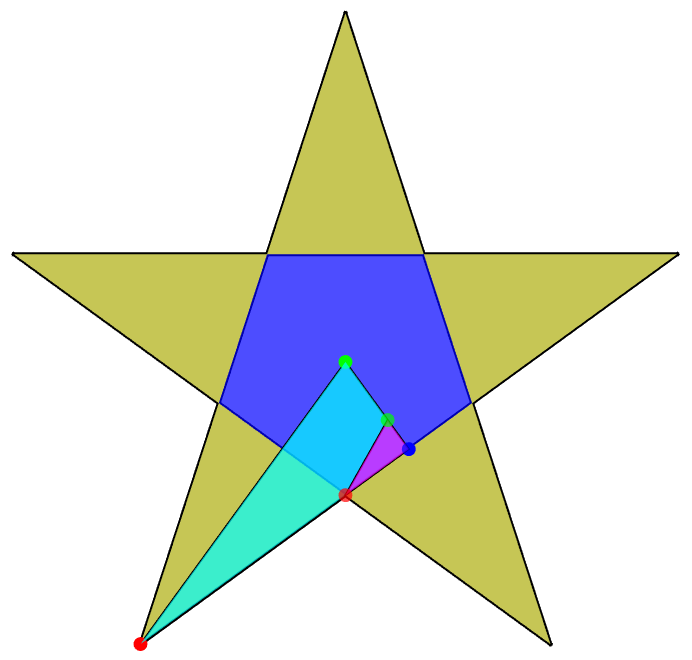
\includegraphics[width=0.8\linewidth]{fig3a}
			\caption{The base face. We also show the base face of $\left\{5,3,\frac{5}{2}\right\}$}\label{fig:13a}
		\end{subfigure}
		\begin{subfigure}{\linewidth}
			\centering
			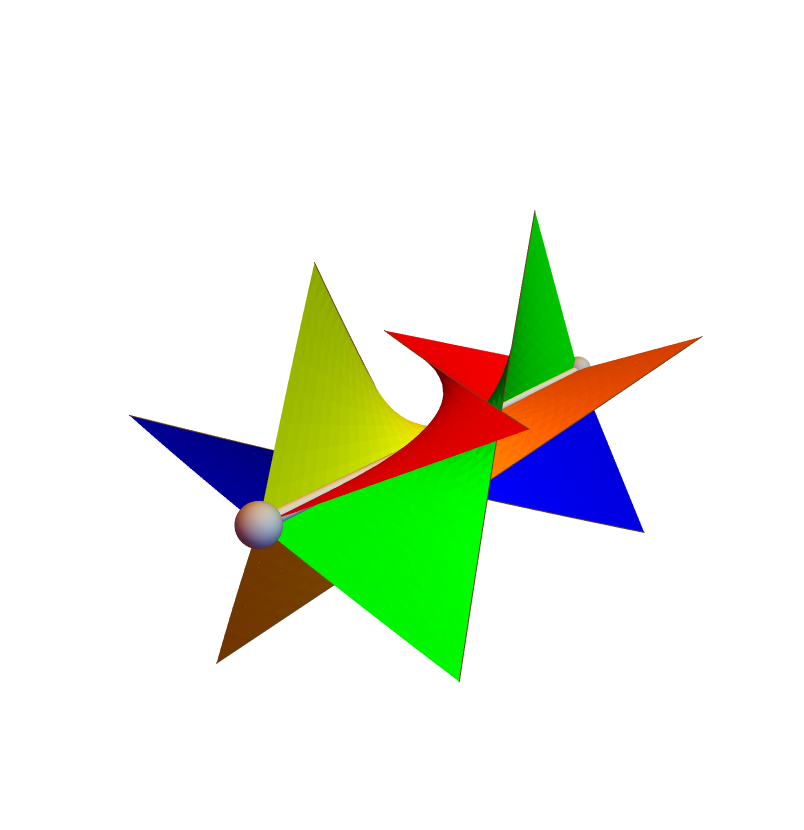
\includegraphics[width=0.5\linewidth]{fig3b}
			\caption{Five faces at the edge. We show part of the surface spanned between the edge and the axis of the twist in every face.}\label{fig:13b}
		\end{subfigure}
	\end{center}
	\caption{Stereographic projections of  $\left\{\frac{12}{1,5},3,\frac{5}{2}\right\}$.}\label{fig:13}
\end{figure}

\clearpage
\begin{appendices}
\crefalias{section}{appendix}
\crefalias{subsection}{appendix}
\section{}\label{app:A}
The original code for the programs used in this thesis may be consulted at \linebreak \href{https://github.com/dan-gc/tesina}{github.com/dan-gc/tesina}.

In the following two sections we show the output of the files \texttt{abstract.txt} and \texttt{geometric.txt} as executed in GAP, in which the abstract and geometric polytopes associated to $\left\{\frac{5}{2},3,5\right\}$ are constructed. The intersection property of $\left\{\frac{5}{2},3,5\right\}$ was confirmed in another program named \texttt{int-prop.txt}, and the constructions regarding $\left\{5,3,\frac{5}{2}\right\}$ are found in analogue programs tagged with the word \texttt{dual}. 

\subsection{\texttt{abstract.txt}}\label{app:1}

\begin{changemargin}{-2cm}{-2cm}
\begin{multicols}{2}
\begin{lstlisting}
	-------------------------------
	ABSTRACT POLYTOPES
	-------------------------------
	
	-------------------------------
	STRING RELATIONS OF {5/2,3,5}
	|<P0>|=2
	|<P1>|=2
	|<P2>|=2
	|<P3>|=2
	
	|<P0*P1>|=5
	|<P1*P2>|=3
	|<P2*P3>|=5
	
	|<P0*P2>|=2
	|<P0*P3>|=2
	|<P1*P3>|=2
	
	Are the groups of {3,3,5} and {5/2,3,5} the same? true
	
	
	-------------------------------
	FACE COUNT OF THE THREE POLYTOPES
	
	{3,3,5}
	
	Vertices in the face: 3
	Vertices in the cell: 4
	Vertices in the polytope: 120
	Edges in the face: 3
	Edges in the cell: 6
	Edges in the polytope: 720
	Faces in the cell: 4
	Faces in the polytope: 1200
	Cells in the polytope: 600
	
	
	{5/2,3,5}
	
	Vertices in the face: 5
	Vertices in the cell: 20
	Vertices in the polytope: 120
	Edges in the face: 5
	Edges in the cell: 30
	Edges in the polytope: 720
	Faces in the cell: 12
	Faces in the polytope: 720
	Cells in the polytope: 120
	
	
	Chiral
	
	Vertices in the cell: 48
	Vertices in the polytope: 120
	Edges in the cell: 72
	Edges in the polytope: 720
	Faces in the cell: 12
	Faces in the polytope: 300
	Cells in the polytope: 50
		\end{lstlisting}
\vfill\null\columnbreak
\begin{lstlisting}
	-------------------------------
	STRING RELATIONS OF CHIRAL
	
	|<S1>|=12
	|<S2>|=3
	|<S3>|=5
	
	|<S1*S2>|=2
	|<S1*S2*S3>|=2
	|<S2*S3>|=2
	
	
	-------------------------------
	INTERSECTION PROPERTY OF CHIRAL
	
	<S1>INT<S2>==<1>  true
	<S2>INT<S3>==<1>  true
	<S1,S2>INT<S2,S3>==<S2>  true
	
	\end{lstlisting}
	\vfill\null\columnbreak
	\begin{lstlisting}
	-------------------------------
	COMBINATORIALLY CHIRAL
	
	Is there an automorphism that satisfies eq. (3)?
	
	rho(S1)=S1^-1  true
	rho(S2)=S1^2*S2  true
	
	Can we extend it to the whole group?  fail
\end{lstlisting}
\end{multicols}
\end{changemargin}

\subsection{\texttt{geometric.txt}}\label{app:2}
\begin{changemargin}{-2cm}{-2cm} 
\begin{multicols}{2}
\begin{lstlisting}
	-------------------------------
	GEOMETRIC POLYTOPES
	-------------------------------
	
	-------------------------------
	STRING RELATIONS OF {5/2,3,5} 
	|<P0>|=2
	|<P1>|=2
	|<P2>|=2
	|<P3>|=2
	
	|<P0*P1>|=5
	|<P1*P2>|=3
	|<P2*P3>|=5
	
	|<P0*P2>|=2
	|<P0*P3>|=2
	|<P1*P3>|=2
	
	Are the groups of {3,3,5} and {5/2,3,5} the same? true
	
	
	-------------------------------
	BASE VERTEX OF {5/2,3,5}
	
	w0P0=w0 false
	w0P1=w0 true
	w0P2=w0 true
	w0P3=w0 true
	
	-------------------------------
	FACE COUNT FOR THE THREE POLYTOPES
	
	{3,3,5}
	
	Vertices in the face: 3
	Vertices in the cell: 4
	Vertices in the polytope: 120
	Edges in the face: 3
	Edges in the cell: 6
	Edges in the polytope: 720
	Faces in the cell: 4
	Faces in the polytope: 1200
	Cells in the polytope: 600
	
	
	{5/2,3,5}
	
	Vertices in the face: 5
	Vertices in the cell: 20
	Vertices in the polytope: 120
	Edges in the face: 5
	Edges in the cell: 30
	Edges in the polytope: 720
	Faces in the cell: 12
	Faces in the polytope: 720
	Cells in the polytope: 120
	
	Chiral
	
	Vertices in the face: 12
	Vertices in the cell: 48
	Vertices in the polytope: 120
	Edges in the face: 12
	Edges in the cell: 72
	Edges in the polytope: 720
	Faces in the cell: 12
	Faces in the polytope: 300
	Cells in the polytope: 50
	
	-------------------------------
	STRING RELATIONS OF CHIRAL
	|<S1>|=12
	|<S2>|=3
	|<S3>|=5
	
	|<S1*S2>|=2
	|<S1*S2*S3>|=2
	|<S2*S3>|=2
	
	
	\end{lstlisting}
	\vfill\null\columnbreak
	\begin{lstlisting}
	-------------------------------
	STABILIZERS OF CHIRAL
	
	S3 fixes the base vertex and edge?
	
	w0.S3=w0  true
	w0.S1^-1.S3=w0.S1^-1  true

	Stabilizers within the cell
	
	Stab_<S1,S2>w0=<S2>  true
	Stab_<S1,S2>e=<S1*S2>  true
	Stab_<S1,S2>f=<S1>  true
	
	
	Stabilizers within the whole polytope
	
	Stab_<S1,S2,S3>w0=<S2,S3>  true
	Stab_<S1,S2,S3>e=<S1*S2,S3>  true
	Stab_<S1,S2,S3>f=<S1,S2*S3>  true
	Stab_<S1,S2,S3>c=<S1,S2>  true
\end{lstlisting}
\end{multicols}
\end{changemargin}
\vspace{-1cm}

\section{}\label{app:coords}
%We show the coordinates as computed in \texttt{Section-5C.nb}. 
In this appendix we show the coordinates of geometric realizations. Let $\phi$ be the golden ratio. As in \cite{petcox}, take the base flag of $\{3,3,5\}$ given by the centroids of the base vertex, edge, face and cell by
\[v_0=(1, 0, 0, 0),\quad v_1=\left(\phi+2,1,0,\frac{1}{\phi }\right), \quad v_2=\left(\phi,\frac{1}{\phi },0,0\right),\quad v_3=\left(\phi ^2,1,-\frac{1}{\phi ^2},0\right),\]
respectively. Then the coordinates of the base vertex of $\left\{\frac{5}{2},3,5\right\}$ are
\[w_0=\left(\frac{\phi }{2}, -\frac{1}{2}, 0, -\frac{1}{2 \phi }\right).\]
according to $w_0=v_0R_0R_1R_2R_1R_2R_3R_2R_1 R_3R_2R_3R_2R_1R_2R_3R_2R_1$, which was found geometrically (see \texttt{52-3-5.nb} for a detailed account). The centroid of the base cell (and hence the base vertex of the dual $\left\{5,3,\frac{5}{2}\right\}$) has coordinates
\[w_3=\left(\frac{\phi }{4}, \frac{1}{4}, 0,-\frac{1}{4 \phi }\right).\]
%The $S_i$ for $\left\{\frac{5}{2},3,5\right\}$ have coordinates
%\[
%	S_1=\frac{1}{2}\left(
%	\begin{array}{cccc}
%		1 & 1 & 1 & -1 \\
%		\phi  & -1 & 0 & \frac{1}{\phi } \\
%		-\frac{1}{\phi } & -1 & \phi  & 0 \\
%		0 & -1 & -\frac{1}{\phi } & -\phi  \\
%	\end{array}	\right),
%	\qquad S_2=\frac{1}{2}\left(
%	\begin{array}{cccc}
%		\phi  & 0 & -\frac{1}{\phi } & -1 \\
%		0 & 2 & 0 & 0 \\
%		\frac{1}{\phi } & 0 & -1 & \phi  \\
%		-1 & 0 & -\phi  & -\phi{1}{\ } \\
%	\end{array}
%	\right),
%\]\[
%	S_3=\frac{1}{2}\left(
%	\begin{array}{cccc}
%		2 & 0 & 0 & 0 \\
%		0 & \phi  & 1 & \frac{1}{\phi } \\
%		0 & -1 & \frac{1}{\phi } & \phi  \\
%		0 & \frac{1}{\phi } & -\phi  & 1 \\
%	\end{array}
%	\right)
%\]
\end{appendices}

\section*{Bibliography}
\addcontentsline{toc}{section}{Bibliography}

\printbibliography[heading=none]
\end{document}